\section{Model pre-processing}

\paragraph*{Inclination}
For non-stationary processes, a method to achieve stationarity involves:
\begin{enumerate}
    \item Identifying and quantifying any clear drift present in the time series by computing the angle of the drift.
    \item Removing the drift from the data.
\end{enumerate}
This process transforms a non-stationary process into a stationary one.
\begin{figure}[H]
    \centering
    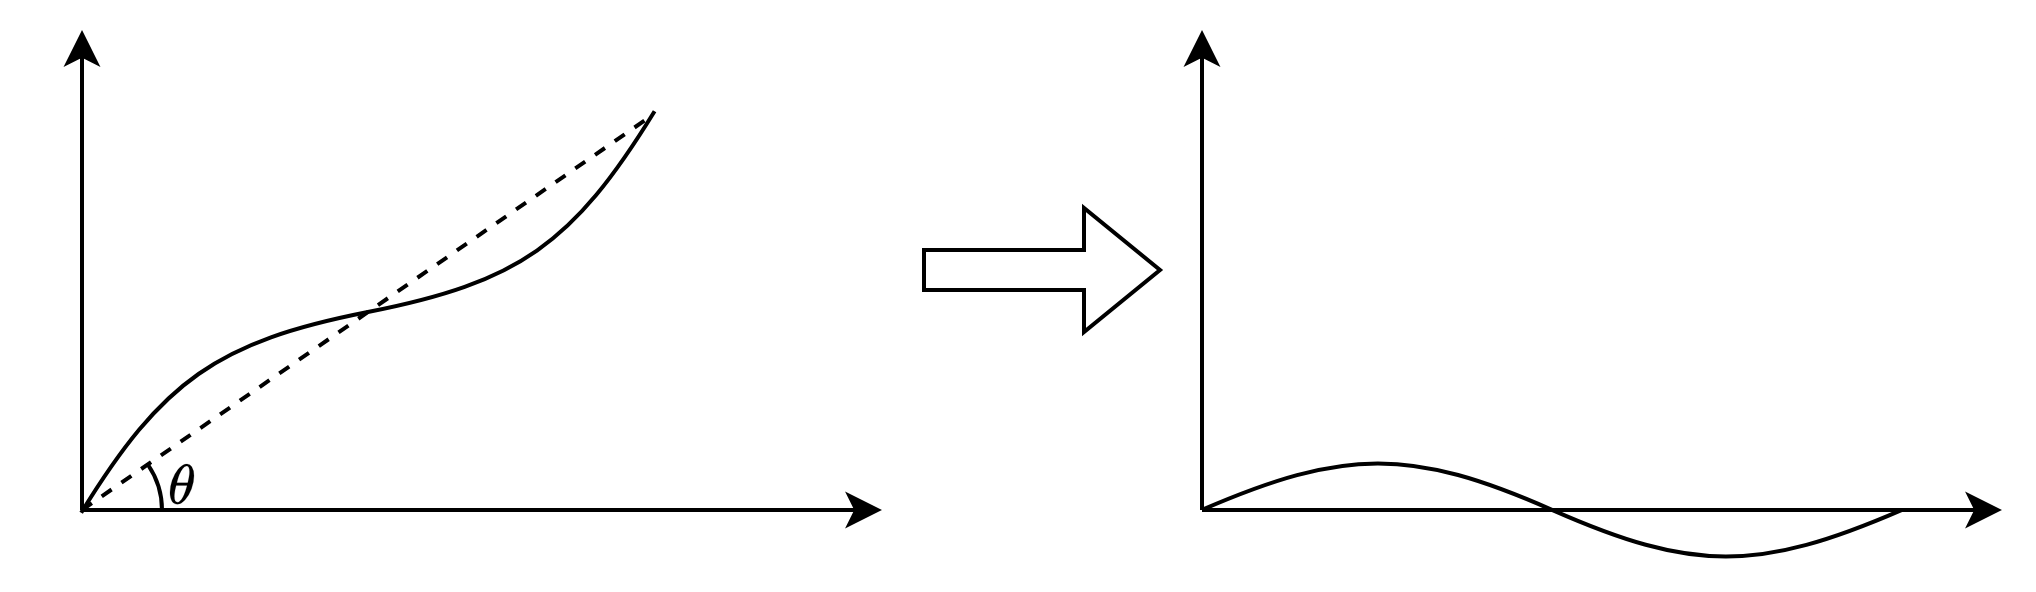
\includegraphics[width=0.75\linewidth]{images/stat.png}
    \caption{Non-stationary process to stationary process}
\end{figure}
Since the drift may not be readily predictable, decomposing the process into a trend and a stationary stochastic process is necessary. 
Subsequently, the trend can be eliminated. 
If the trend follows a linear expression, such as $kt+q$, where $k$ and $q$ are parameters, the expectation of the process can be expressed as:
\[\mathbb{E}\left[y(t)\right]=\mathbb{E}\left[y^\prime(t)-kt-q\right]=0\]
Following this, the least squares problem can be formulated to minimize:
\[\min_{k,q}\dfrac{1}{N}\sum_{t=1}^{N}\left(y^\prime(t)-kt-q\right)^2\]
Upon solving this problem, estimates for $\hat{k}$ and $\hat{q}$ are obtained.

\paragraph*{Seasonality}
For processes exhibiting seasonality, in addition to trends, we may encounter periodic variations. 
To handle seasonality, the process can be decomposed into a seasonal component $s(t)$ and a stationary stochastic process.

Determining the period of seasonality, denoted as $T$, is crucial. 
It represents the duration after which the seasonality pattern repeats:
\[s(t)=s(t+Kt)\qquad k \in \mathbb{Z}\]
The period $T$ can be identified by examining the frequency domain and identifying the highest frequency, then computing its inverse.

Once the period $T$ is determined, we can aggregate observations occurring at the same time within each period. 
This involves averaging all observations at corresponding time instants across multiple periods:
\[\hat{s}(t)=\dfrac{1}{M}\sum_{h=1}^{M}y(t+hT)\qquad t=1,2,\dots,N\]
Here, $M$ represents the number of periods observed in the dataset.
This averaging process yields an estimate for $s(t)$ at each time instant within the season.